\section{Test Cases and Results}
\label{sec:results}

\subsection{Tunnel}
\label{sec:particleTunnel}

The tunnel test case is very simple and was mainly used for debugging during development. It consists of ten cubes. This is illustrated in figure \ref{fig:particleTunnel} the particles are colored by the x-coordinate (goes from left to right in the illustration) of their velocity.

\textbf{\begin{figure}[H]
  \centering
  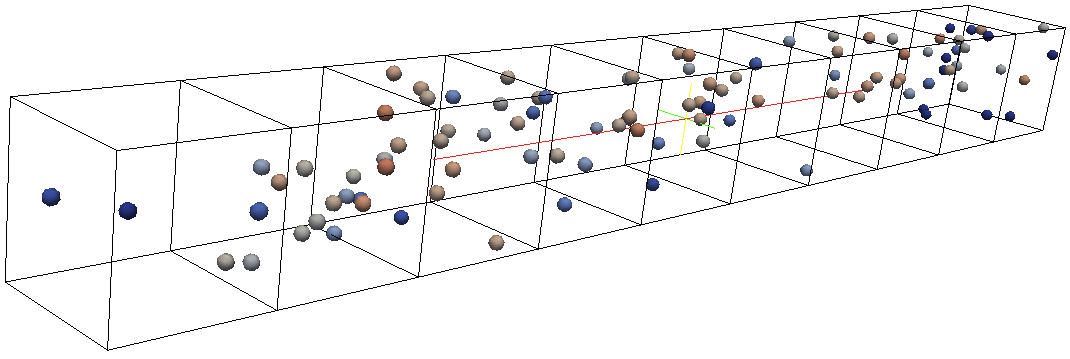
\includegraphics[scale=0.4]{content/gfx/particleTunnel.png}
  \caption{Particle tunnel with randomly distributed particles.}
  \label{fig:particleTunnel}
\end{figure}}

\subsection{Torus}
\label{sec:torus}

The second test case is a simple torus. A torus is defined by two circles orthogonal to each other in three dimensional space. The smaller circle is then rotated around the bigger circle leading to a surface of revolution which defines the torus.

\textbf{\begin{figure}[H]
  \centering
  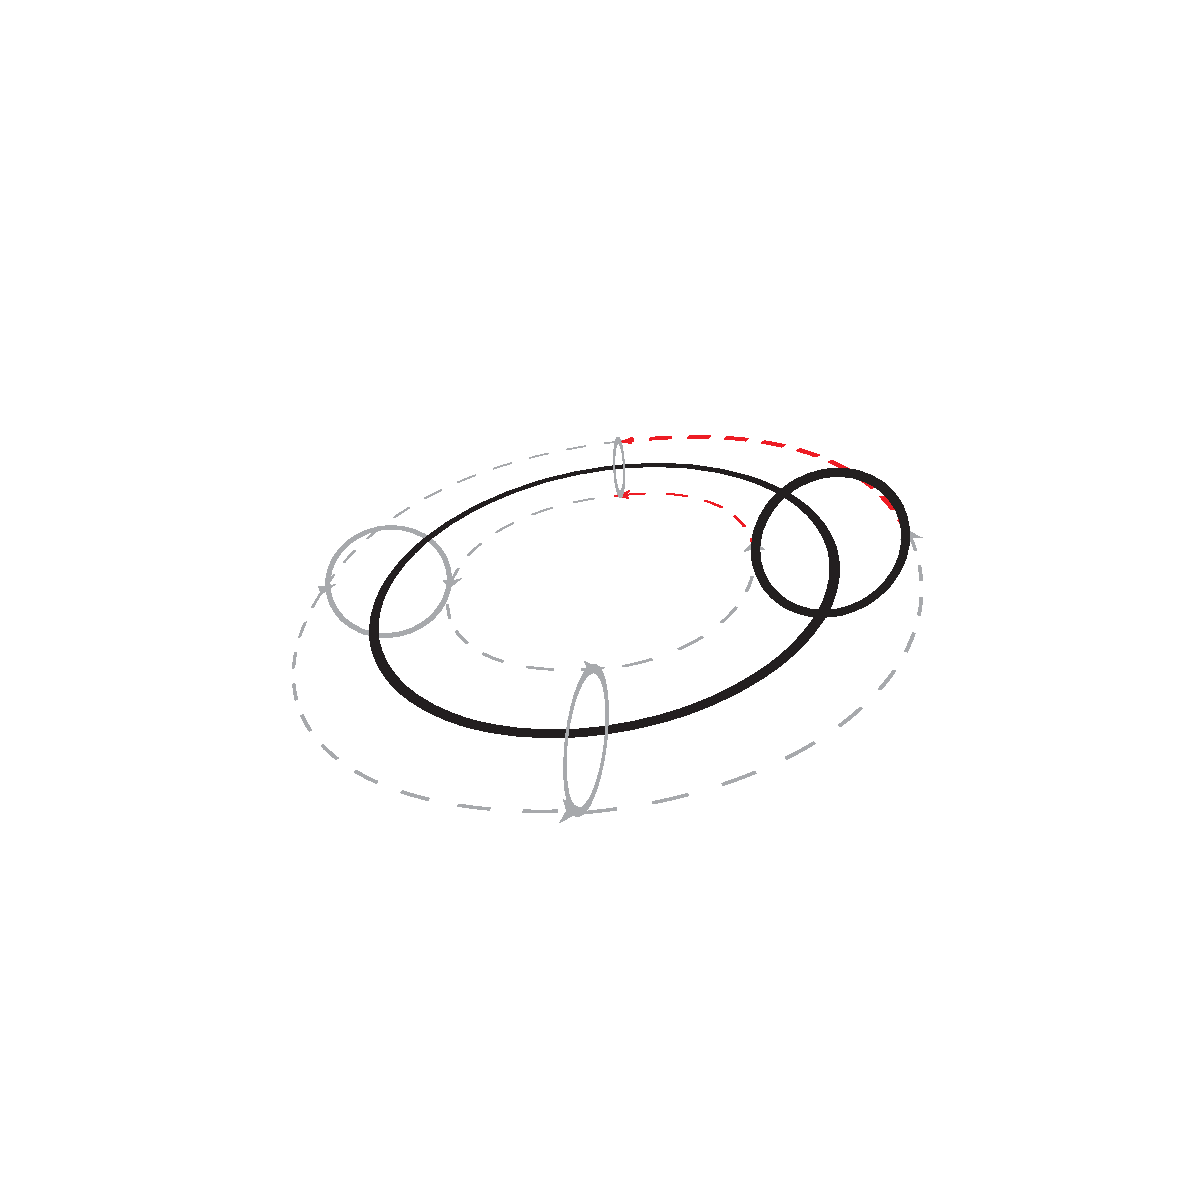
\includegraphics[scale=0.8]{content/gfx/torus.pdf}
  \caption{A torus defined by surface revolution of a circle.}
  \label{fig:torus}
\end{figure}}

In order to polygonally approximate the torus discrete points on the rotating circle are calculated using formula \ref{eq:torus}. The formula requires the following parameters: $(x_0, y_0)$ is the center of the circle, $r$ is the radius of the circle and $(x, y)$ the points lying on the circle.

\begin{equation}
    \label{eq:torus}
    (x, y) = (x_0 + r \cdot cos(\alpha), y_0 + r \cdot sin(\alpha))
\end{equation}

% TODO figure explaining the discretisation

The mesh was then generated using netgen \cite{netgen}, a simple mesh generator which can export meshes in the OpenFOAM format.

\textbf{\begin{figure}[H]
  \centering
  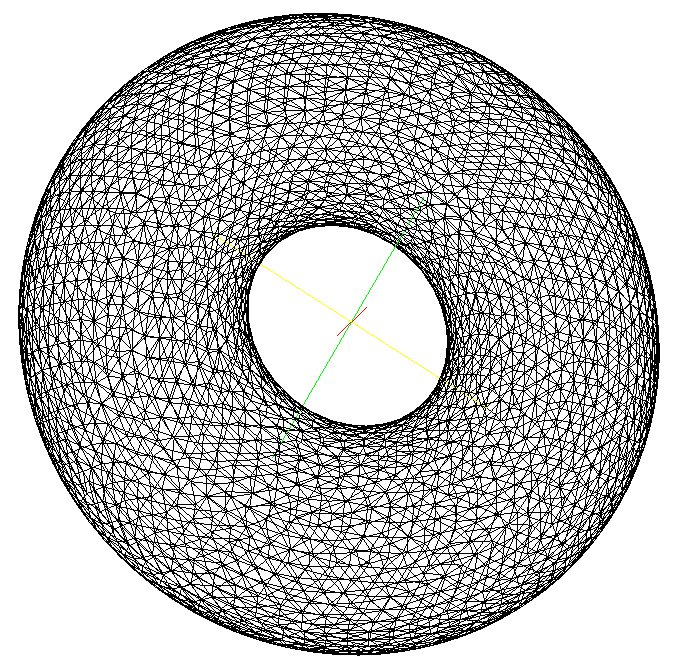
\includegraphics[scale=0.4]{content/gfx/torusCoarseMesh.png}
  \caption{A tetrahedral mesh generated in a torus.}
  \label{gfx:torus}
\end{figure}}

Figure \ref{gfx:torus} shows a coarse mesh with around 30000 cells generated in  a torus.

\subsection{Measurements}

The performance measurements are done using the torus case with 228'184 cells. The tests ran on an Intel 655k CPU\footnote{\url{http://ark.intel.com/Product.aspx?id=48750}} and an Nvidia GeForce GTX 470\footnote{\url{http://www.nvidia.com/object/product_geforce_gtx_470_us.html}}. Both parts have been released to the market in 2010. 50'000 particles are tracked over ten time steps, which is equivalent to calculating the lambdas for 500'000 particles.

\begin{table}[H]
    \centering
    \begin{tabular}{| l | l | l |}
        \hline
                          & \textbf{CPU} & \textbf{GPU} \\ \hline
        Single Precision  & 2'810'792    &  220'866 \\ \hline
        Double Precision  & 3'264'259    &  376'349 \\ \hline
    \end{tabular}
    \caption{Execution time in microseconds}
    \label{table:execTime}
\end{table}

Table \ref{table:execTime} compares the time required to calculate the lambdas on the CPU using the OpenFOAM code and on the GPU using the code developed during this thesis. It should be noted that the GPU time includes the time required to copy all the data over the PCI bus and that the actual computing time on the GPU is much shorter! Because of this tracking particles on the GPU only makes sense for a larger number of particles as illustrated by figure \ref{gfx:plotGpuVSCpu}. 

\textbf{\begin{figure}[H]
  \centering
  % GNUPLOT: LaTeX picture with Postscript
\begingroup
  \makeatletter
  \providecommand\color[2][]{%
    \GenericError{(gnuplot) \space\space\space\@spaces}{%
      Package color not loaded in conjunction with
      terminal option `colourtext'%
    }{See the gnuplot documentation for explanation.%
    }{Either use 'blacktext' in gnuplot or load the package
      color.sty in LaTeX.}%
    \renewcommand\color[2][]{}%
  }%
  \providecommand\includegraphics[2][]{%
    \GenericError{(gnuplot) \space\space\space\@spaces}{%
      Package graphicx or graphics not loaded%
    }{See the gnuplot documentation for explanation.%
    }{The gnuplot epslatex terminal needs graphicx.sty or graphics.sty.}%
    \renewcommand\includegraphics[2][]{}%
  }%
  \providecommand\rotatebox[2]{#2}%
  \@ifundefined{ifGPcolor}{%
    \newif\ifGPcolor
    \GPcolortrue
  }{}%
  \@ifundefined{ifGPblacktext}{%
    \newif\ifGPblacktext
    \GPblacktexttrue
  }{}%
  % define a \g@addto@macro without @ in the name:
  \let\gplgaddtomacro\g@addto@macro
  % define empty templates for all commands taking text:
  \gdef\gplbacktext{}%
  \gdef\gplfronttext{}%
  \makeatother
  \ifGPblacktext
    % no textcolor at all
    \def\colorrgb#1{}%
    \def\colorgray#1{}%
  \else
    % gray or color?
    \ifGPcolor
      \def\colorrgb#1{\color[rgb]{#1}}%
      \def\colorgray#1{\color[gray]{#1}}%
      \expandafter\def\csname LTw\endcsname{\color{white}}%
      \expandafter\def\csname LTb\endcsname{\color{black}}%
      \expandafter\def\csname LTa\endcsname{\color{black}}%
      \expandafter\def\csname LT0\endcsname{\color[rgb]{1,0,0}}%
      \expandafter\def\csname LT1\endcsname{\color[rgb]{0,1,0}}%
      \expandafter\def\csname LT2\endcsname{\color[rgb]{0,0,1}}%
      \expandafter\def\csname LT3\endcsname{\color[rgb]{1,0,1}}%
      \expandafter\def\csname LT4\endcsname{\color[rgb]{0,1,1}}%
      \expandafter\def\csname LT5\endcsname{\color[rgb]{1,1,0}}%
      \expandafter\def\csname LT6\endcsname{\color[rgb]{0,0,0}}%
      \expandafter\def\csname LT7\endcsname{\color[rgb]{1,0.3,0}}%
      \expandafter\def\csname LT8\endcsname{\color[rgb]{0.5,0.5,0.5}}%
    \else
      % gray
      \def\colorrgb#1{\color{black}}%
      \def\colorgray#1{\color[gray]{#1}}%
      \expandafter\def\csname LTw\endcsname{\color{white}}%
      \expandafter\def\csname LTb\endcsname{\color{black}}%
      \expandafter\def\csname LTa\endcsname{\color{black}}%
      \expandafter\def\csname LT0\endcsname{\color{black}}%
      \expandafter\def\csname LT1\endcsname{\color{black}}%
      \expandafter\def\csname LT2\endcsname{\color{black}}%
      \expandafter\def\csname LT3\endcsname{\color{black}}%
      \expandafter\def\csname LT4\endcsname{\color{black}}%
      \expandafter\def\csname LT5\endcsname{\color{black}}%
      \expandafter\def\csname LT6\endcsname{\color{black}}%
      \expandafter\def\csname LT7\endcsname{\color{black}}%
      \expandafter\def\csname LT8\endcsname{\color{black}}%
    \fi
  \fi
  \setlength{\unitlength}{0.0500bp}%
  \begin{picture}(7200.00,5040.00)%
    \gplgaddtomacro\gplbacktext{%
      \csname LTb\endcsname%
      \put(1474,704){\makebox(0,0)[r]{\strut{} 0}}%
      \put(1474,1229){\makebox(0,0)[r]{\strut{} 500000}}%
      \put(1474,1754){\makebox(0,0)[r]{\strut{} 1e+06}}%
      \put(1474,2279){\makebox(0,0)[r]{\strut{} 1.5e+06}}%
      \put(1474,2804){\makebox(0,0)[r]{\strut{} 2e+06}}%
      \put(1474,3329){\makebox(0,0)[r]{\strut{} 2.5e+06}}%
      \put(1474,3854){\makebox(0,0)[r]{\strut{} 3e+06}}%
      \put(1474,4379){\makebox(0,0)[r]{\strut{} 3.5e+06}}%
      \put(1606,484){\makebox(0,0){\strut{} 0}}%
      \put(2126,484){\makebox(0,0){\strut{} 5}}%
      \put(2645,484){\makebox(0,0){\strut{} 10}}%
      \put(3165,484){\makebox(0,0){\strut{} 15}}%
      \put(3685,484){\makebox(0,0){\strut{} 20}}%
      \put(4205,484){\makebox(0,0){\strut{} 25}}%
      \put(4724,484){\makebox(0,0){\strut{} 30}}%
      \put(5244,484){\makebox(0,0){\strut{} 35}}%
      \put(5764,484){\makebox(0,0){\strut{} 40}}%
      \put(6283,484){\makebox(0,0){\strut{} 45}}%
      \put(6803,484){\makebox(0,0){\strut{} 50}}%
      \put(176,2541){\rotatebox{-270}{\makebox(0,0){\strut{}Time in Microseconds}}}%
      \put(4204,154){\makebox(0,0){\strut{}Number of Particles (times 10'000)}}%
      \put(4204,4709){\makebox(0,0){\strut{}CPU vs GPU}}%
    }%
    \gplgaddtomacro\gplfronttext{%
      \csname LTb\endcsname%
      \put(5816,4206){\makebox(0,0)[r]{\strut{}CPU}}%
      \csname LTb\endcsname%
      \put(5816,3986){\makebox(0,0)[r]{\strut{}GPU}}%
    }%
    \gplbacktext
    \put(0,0){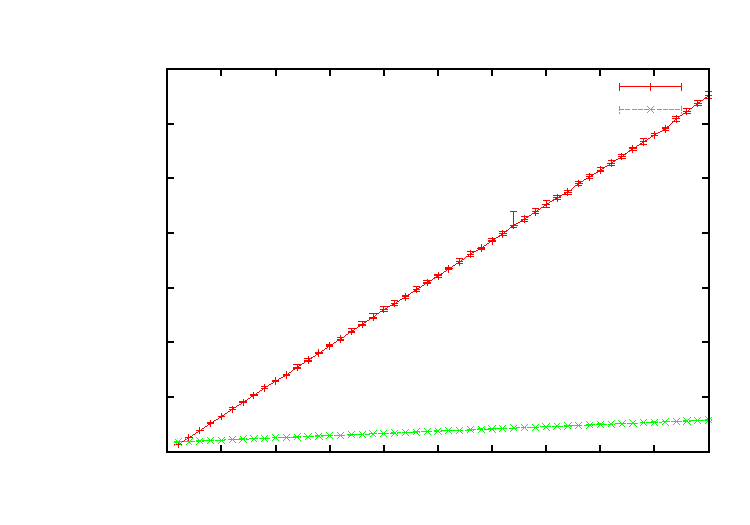
\includegraphics{content/gfx/gpuVsCpu}}%
    \gplfronttext
  \end{picture}%
\endgroup

  \caption{Plot showing the execution time for a growing number of particles.}
  \label{gfx:plotGpuVSCpu}
\end{figure}}

The execution times in figure \ref{gfx:plotGpuVSCpu} have been measured ten times at each point. For each point the average, the highest and lowest time is shown, the average values are connected by lines. As one can see there are some measurement errors on the CPU, this is most likely because the operating system and further user processes are running on the CPU along with the OpenFOAM code. On the GPU only very little diversity in the measurements can be seen, this is because the test was running on a dedicated GPU, not used for graphics.

For a more detailed analysis of the computing time spent on the GPU Nvidia's Compute Profiler \cite{computeprof} was used.

\textbf{\begin{figure}[H]
  \centering
  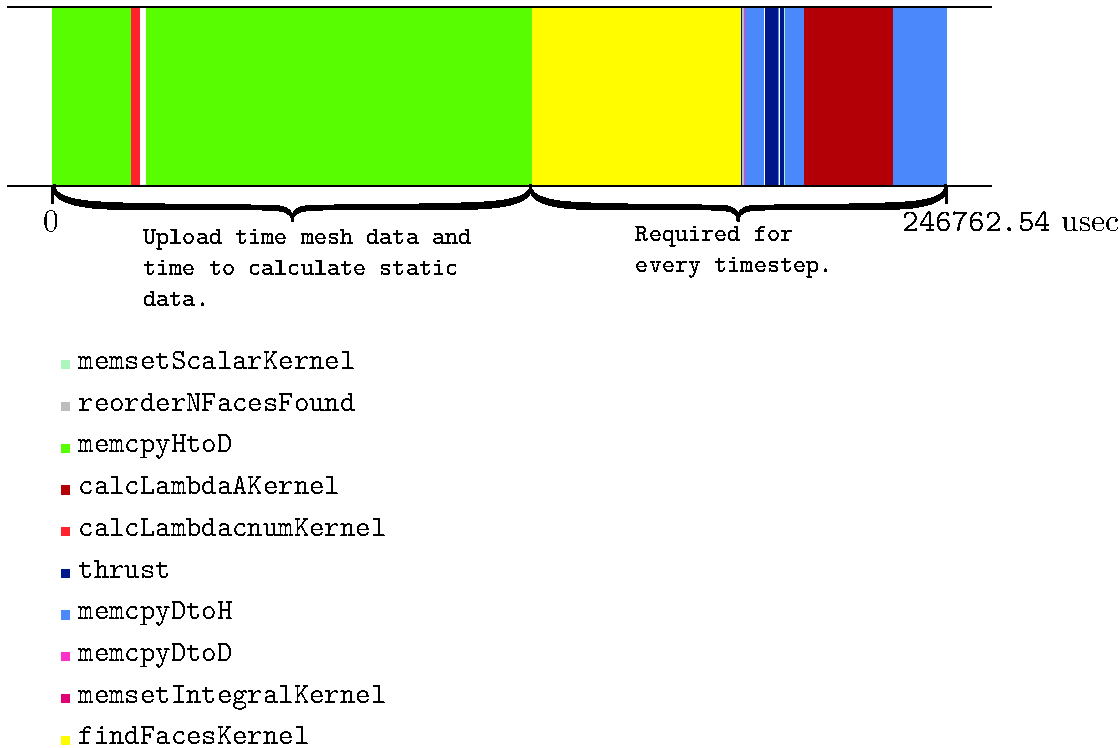
\includegraphics[scale=0.6]{content/gfx/widthPlot1.pdf}
  \caption{Width plot showing the time of kernel functions and memcpy operations.}
  \label{fig:widthPlot}
\end{figure}}

Figure \ref{fig:widthPlot} shows a width plot of the GPU time\footnote{The plot was done using the same test case (with double precision) as presented before in table \ref{table:execTime}. The shorter time is because this is a sum of time measured on the GPU (for copying data and GPU kernels), while the time presented in the table was measured on the CPU and therefore includes overhead for invoking memory copies and GPU kernels.}. The white spaces in between indicate idle time in which the host code is doing something. It can be easily seen that around 60 \% of the run time are memory copying time! Furthermore the first chunk of data copied is the mesh data. This together with the initial calculation must be done only once.

\textbf{\begin{figure}[H]
  \centering
  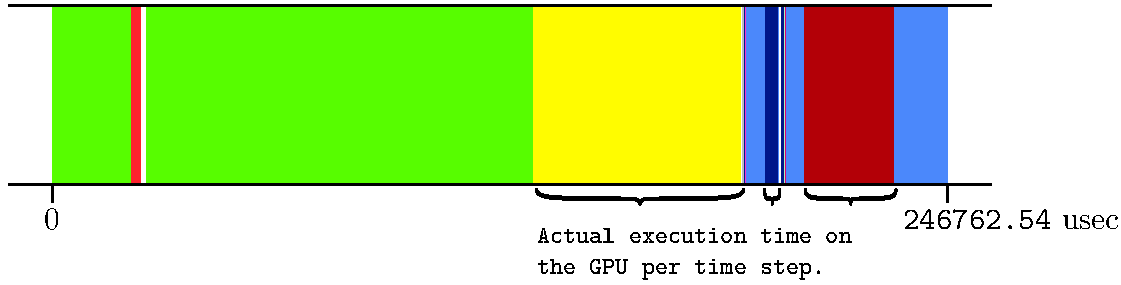
\includegraphics[scale=0.6]{content/gfx/widthPlotAcutalExecutionTimeGPU.pdf}
  \caption{Width plot showing the actual time spent on the GPU.}
  \label{fig:widthPlotAcutalTimeGPU}
\end{figure}}

If we do not consider the time spent to copy the data over the PCI bus and to do the initial calculation, then we get an actual run time on the GPU of just 89'742 usec per time step (double precision). \textit{That is more than 30 times faster than the single threaded CPU implementation.} The actual execution time on the GPU is illustrated in figure \ref{fig:widthPlotAcutalTimeGPU}.

\subsection{Performance Analysis of Computational Kernels}

There are three major kernels involved in the computation: A kernel which calculates the numerator of $\lambda_c$ at the beginning (initial step in figure \ref{gfx:SequenceTracking}), this kernel has one thread per cell. A kernel which finds all faces with $\lambda_c \in [0, 1]$ (step 2 in figure \ref{gfx:SequenceTracking}) with one thread per particle and a kernel which calculates $\lambda_a$ for the particles with $\lambda_c \in [0, 1]$\footnote{The kernels to calculate the lambdas are parallelized over the number of particles. It would also be possible to parallelize over all the cells in the mesh but this would require that each thread iterates over the particles in its cell. Because the number of particles per cell usually varies this would lead to massively divergent warps and therefore poor performance \cite[5.4.2]{cudaguide}} (step 4 in figure \ref{gfx:SequenceTracking}). 

Because the kernel responsible for finding faces with $\lambda_c \in [0,1]$ takes the most time to compute (figure \ref{fig:widthPlot}, yellow) it is analysed here. The structure of the kernel is as follows: First data belonging to the cell and the particle is fetched using the particle label. Then it is iterated over all faces of the cell where first the face data (face normal and face centre) is fetched and then the lambdas are calculated. If they are within the desired interval the label of the face is written into the faces found array. Once the loop is done the number of faces found is written back. When compiled for double precision the kernel's occupancy (see section \ref{sec:gpuArch}) is quite low around 33\%, this is because each thread requires 34 registers. Compiled for single precision improves the occupancy (around 66\%), because just 24 registers are required. In both cases the occupancy is limited by register usage. If it could be done with just 16 registers per thread, the occupancy would be 100 \%. The kernel is memory bound, meaning that execution time is wasted by waiting for data from global memory. The main reason for this are uncoalesced reads and writes as well as the low occupancy. For example writing the face labels found is uncoalesced because it differs for every thread and therefore it is written back sequentially. There are different options to further improve the kernel's efficiency

\begin{itemize}
    \item Turn off L1 cache for global memory access. Uncached memory transactions are multiples of 32, 64 and 128 bytes where cached transactions are always multiples of 128 bytes (the cache line size) \cite[F.4.2]{cudaguide}. In case of uncoalesced memory access, smaller transactions are better, because the full size of the cache line is not used anyways. Quickly trying this out lead to a slight improvement of around 20\%\footnote{The plots presented before are with L1 cache enabled.}.
    \item Use shared memory or texture cache. Shared memory is fast, on-chip memory, which can be accessed by threads in the same block \cite[3.2.3]{cudaguide}. However tracking particles in an unstructured mesh is not well suited for shared memory: Using shared memory requires that threads sharing data are placed in the same CUDA block. The threads for the particles which reside in the same cell share data: The cell centre, face centres and normals, etc. However this would require that the particles are sorted by the occupancy cells. Also all CUDA blocks for a kernel launch must be of the same size. Furthermore the block size should be a multiple of the wrap size (32 threads) and at minimum 64 threads \cite[4.4]{cudaBestPractices}. This makes it unfeasible to use shared memory. Using texture memory \cite[3.2.10.1]{cudaguide} might speed up the kernel, since it lead to significant performance improvement in Nvidia's particle demo (see section \ref{sec:summary}).
    \item Review the code and rearrange data in order to improve memory access patterns and reduce the register requirements. The kernel code first fetches the label of the particles. During the first iteration the label of the particles correspond directly to the thread index. The particle labels array is just used in later iterations, where some particles are already done. Because the number of particles which need to be considered in further iterations are usually much smaller, this could lead to a significant improvement. 
\end{itemize}

\subsection{Memory Requirements}

GPUs have memory buses designed to reduce latency and not to support a very large amount of memory as CPUs do. To day GPUs can have at most 6GB of RAM. For larger cases it is probably required to partition the particles into chunks fitting into the memory of the GPU.

In the simulation code a particle requires about 1338 bytes of memory to store all the relevant data (position, velocity, diameter, label, etc). Therefore processing one million particles at once would require around 1.25 Gb of memory just for the particles. A tetrahedral mesh cell requires about 221 bytes of memory. A mesh with one million cells therefore requires about 212 Mb of data. The \verb+calcLambda+ test program and the \verb+gpuLagrangianFoam+ solver report the data required on the GPU at the beginning of the simulation.